\documentclass[10pt,letterpaper]{article}
\usepackage[utf8]{inputenc}
\usepackage[english]{babel}
\usepackage{amsmath}
\usepackage{amsfonts}
\usepackage{amssymb}

\usepackage{float}
\usepackage{makeidx}

\usepackage{graphicx}
\graphicspath{ {./images/} }

\usepackage{listings}
\usepackage{xcolor}

\definecolor{codegreen}{rgb}{0,0.6,0}
\definecolor{codegray}{rgb}{0.5,0.5,0.5}
\definecolor{codepurple}{rgb}{0.58,0,0.82}
\definecolor{backcolour}{rgb}{0.95,0.95,0.92}

\lstdefinestyle{mystyle}{
    backgroundcolor=\color{backcolour},   
    commentstyle=\color{codegreen},
    keywordstyle=\color{magenta},
    numberstyle=\tiny\color{codegray},
    stringstyle=\color{codepurple},
    basicstyle=\ttfamily\footnotesize,
    breakatwhitespace=false,         
    breaklines=true,                 
    captionpos=b,                    
    keepspaces=true,                 
    numbers=left,                    
    numbersep=5pt,                  
    showspaces=false,                
    showstringspaces=false,
    showtabs=false,                  
    tabsize=2
}
\lstset{style=mystyle}

\usepackage{lmodern}
\usepackage{kpfonts}
\usepackage{comment}
\usepackage{hyperref}
\hypersetup{
    colorlinks=true,
    linkcolor=blue,
    filecolor=magenta,      
    urlcolor=cyan,
    pdftitle={Overleaf Example},
    pdfpagemode=FullScreen,
    }
\usepackage[left=2cm,right=2cm,top=2cm,bottom=2cm]{geometry}
\title{\textbf{Data Scientist Review}}
\author{Ce Peng}
\date{June 22 2021}
\begin{document}
\begin{titlepage}
\maketitle\maketitle
\begin{flushleft}
\href{https://www.overleaf.com/learn}{Latex code ref https://www.overleaf.com/learn} \\
\href{https://stanford.edu/~cpiech/cs221/handouts/kmeans.html}{Algorithm content ref https://stanford.edu/~cpiech/cs221/handouts/kmeans.html}
\end{flushleft}
\end{titlepage}

\subsection{Interview Questions}
\subsubsection{Question 1}
What are drawback of K-means clustering?
\begin{itemize}
\item Outliers need to be removed before clustering as it can tend to include outliers into clusters.
\end{itemize}

\subsubsection{Outlier}

In \href{https://en.wikipedia.org/wiki/Outlier#Identifying_outliers}{Wikipedia},it says that in statistics, an outlier is a data point that differs significantly from other observations.[1][2] An outlier may be due to variability in In statistics, an outlier is a data point that differs significantly from other observations. An outlier may be due to variability in the measurement or it may indicate experimental error; the latter are sometimes excluded from the data set. An outlier can cause serious problems in statistical analyses.

the measurement or it may indicate experimental error; the latter are sometimes excluded from the data set. An outlier can cause serious problems in statistical analyses.

\begin{figure}[H]
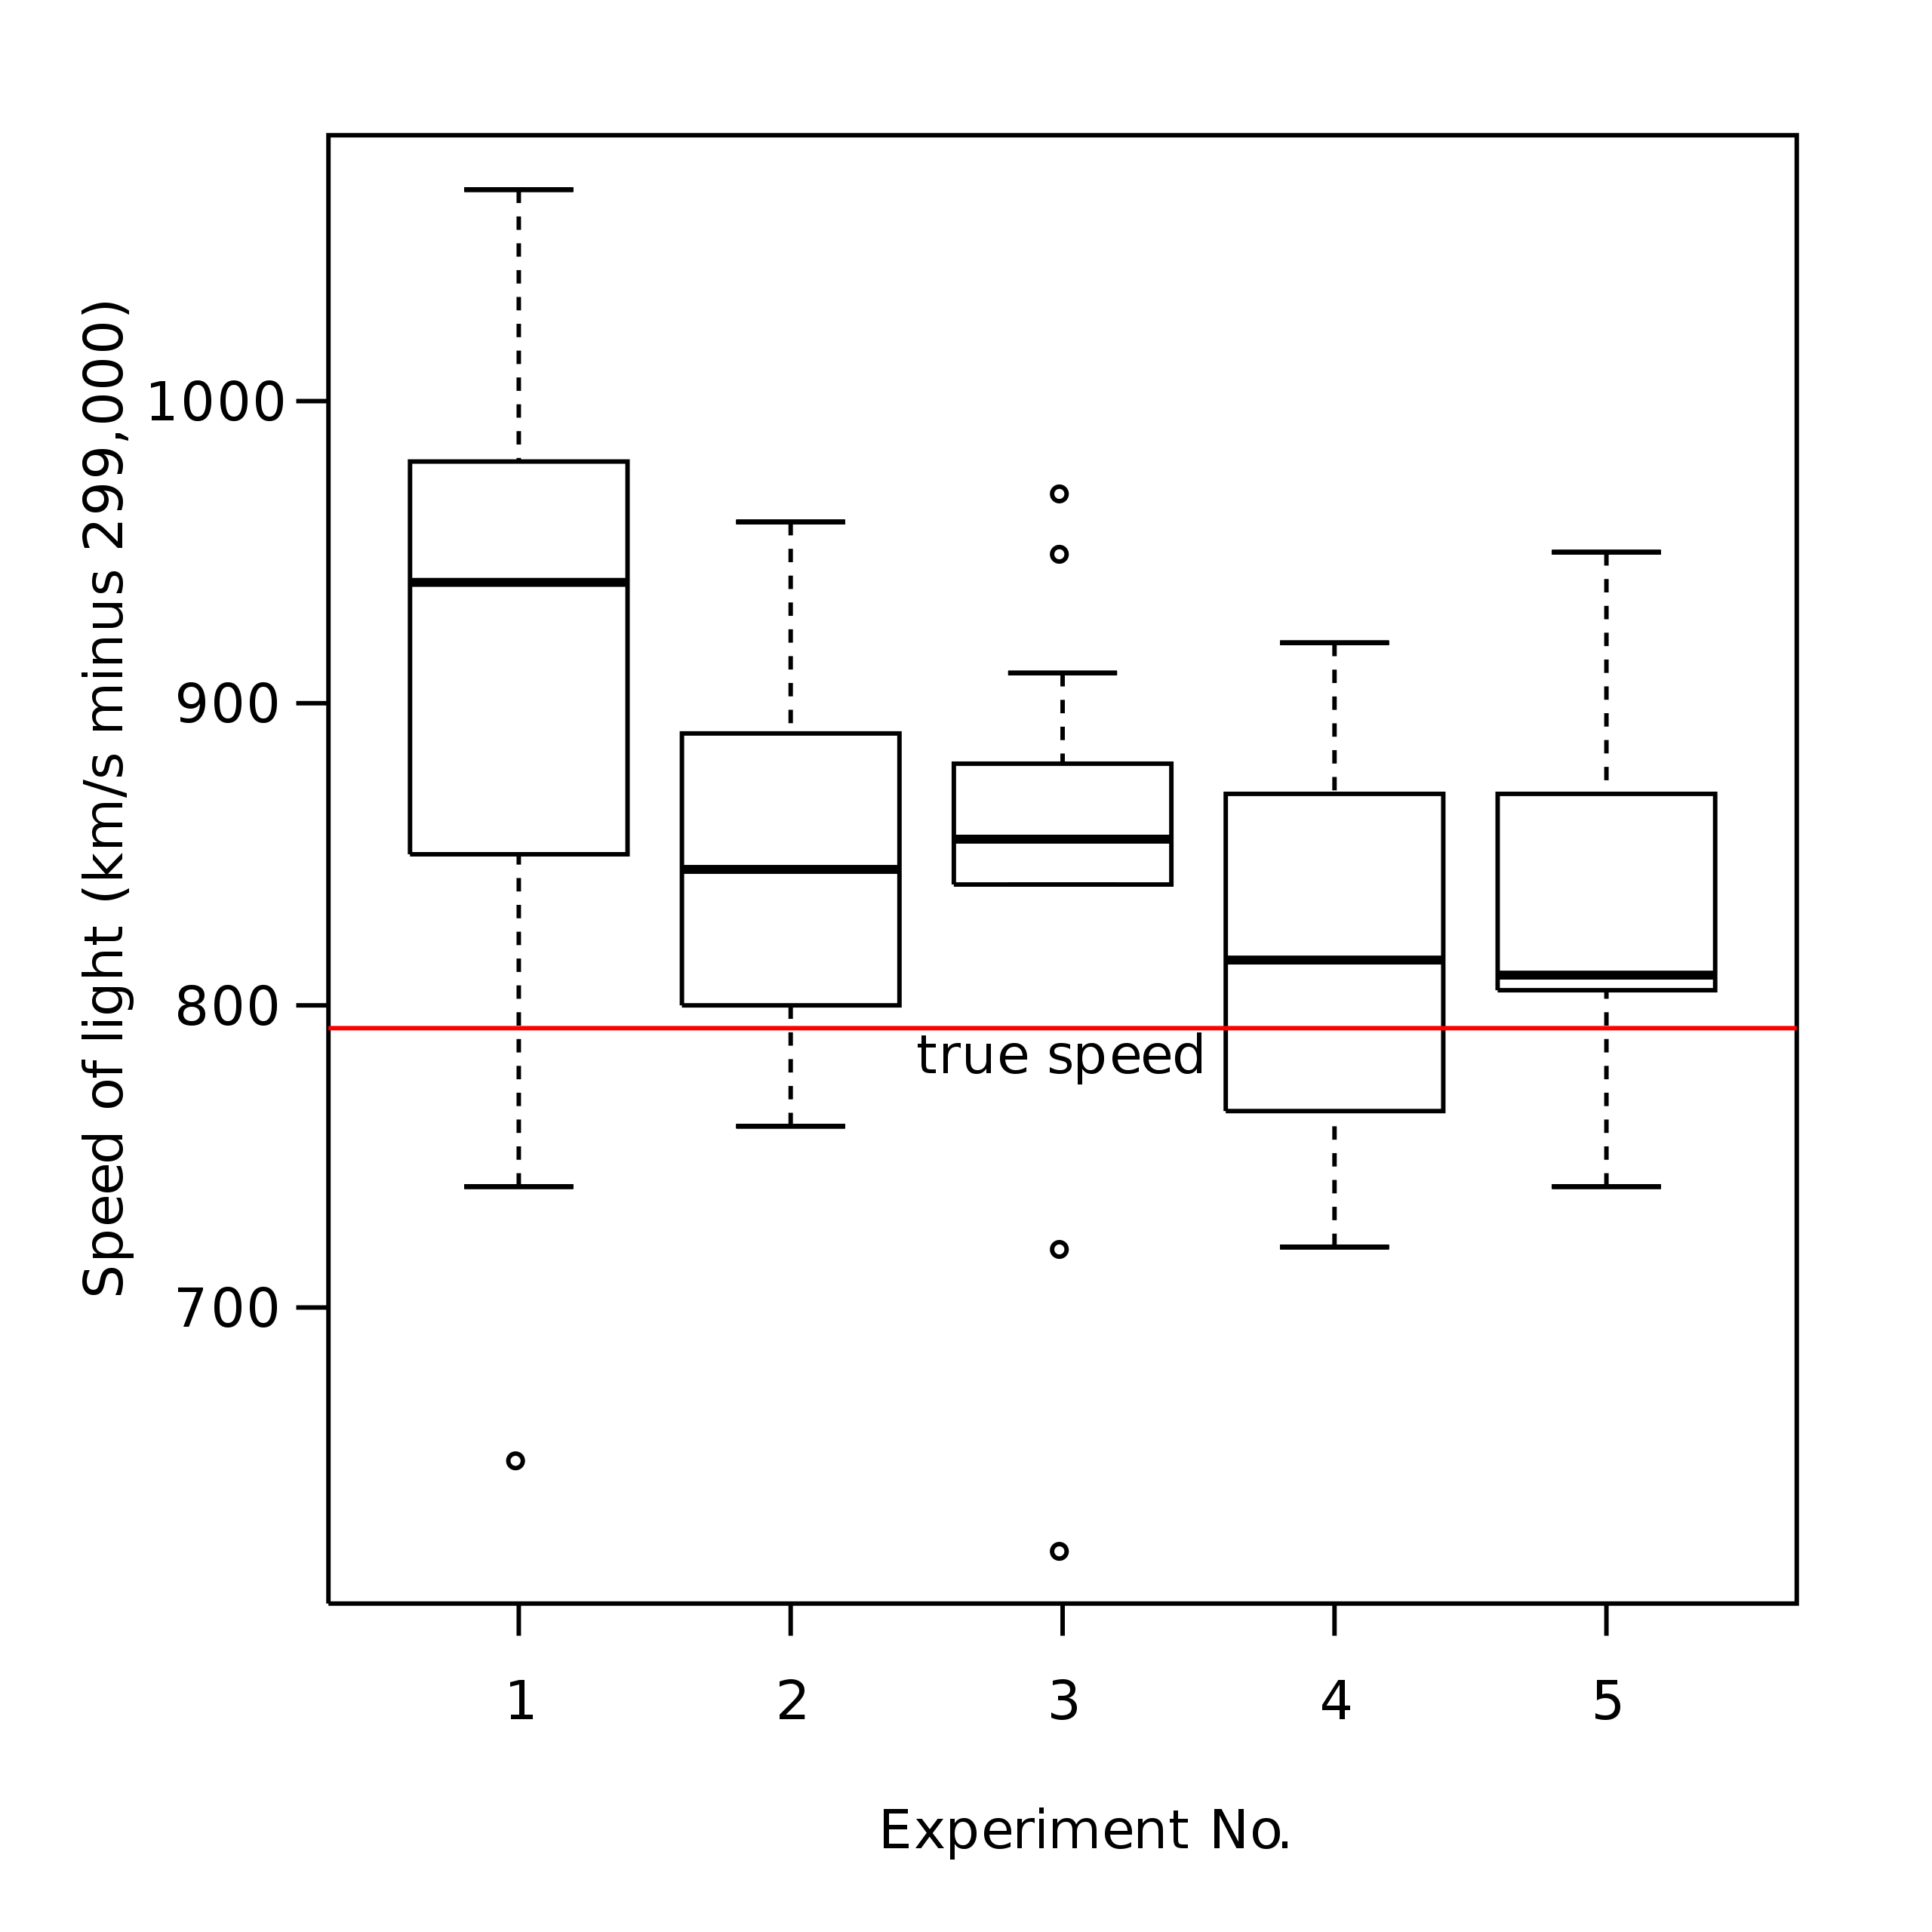
\includegraphics[width=.3\textwidth]{2560px-Michelsonmorley-boxplot.svg.png}
\centering
\caption{ Box plot of data from the Michelson–Morley experiment displaying four outliers in the middle column, as well as one outlier in the first column.}
\label{figure4}
\end{figure}

\section{K-means}
This chapter is written by Chris Piech. Based on a handout by Andrew Ng.
\subsection{Basic Idea}
Say you are given a data set where each observed example has a set of features, but has no labels. Labels are an essential ingredient to a supervised algorithm like Support Vector Machines, which learns a hypothesis function to predict labels given features. So we can't run supervised learning. What can we do? \\

One of the most straightforward tasks we can perform on a data set without labels is to find groups of data in our dataset which are similar to one another -- what we call clusters.\\

K-Means is one of the most popular "clustering" algorithms. K-means stores $k$ centroids that it uses to define clusters. A point is considered to be in a particular cluster if it is closer to that cluster's centroid than any other centroid.\\

K-Means finds the best centroids by alternating between (1) assigning data points to clusters based on the current centroids (2) chosing centroids (points which are the center of a cluster) based on the current assignment of data points to clusters.\\

\begin{figure}[H]
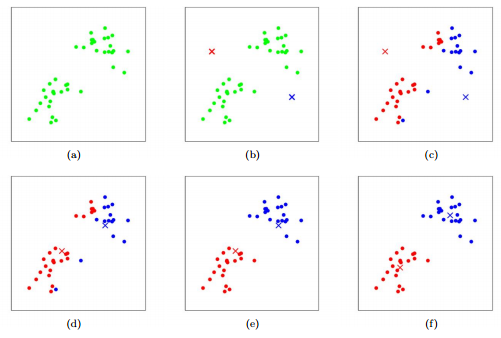
\includegraphics[width=0.8\textwidth]{kmeansViz.png}
\centering
\caption{K-means algorithm. Training examples are shown as dots, and cluster centroids are shown as crosses. (a) Original dataset. (b) Random initial cluster centroids. (c-f) Illustration of running two iterations of k-means. In each iteration, we assign each training example to the closest cluster centroid (shown by "painting" the training examples the same color as the cluster centroid to which is assigned); then we move each cluster centroid to the mean of the points assigned to it. Images courtesy of Michael Jordan.}
\label{figure1}
\end{figure}

\subsection{Algorithm}
In the clustering problem, we are given a training set ${x^{(1)}, ... , x^{(m)}}$, and want to group the data into a few cohesive "clusters." Here, we are given feature vectors for each data point $x^{(i)} \in \mathbb{R}^n$ as usual; but no labels $y^{(i)}$ (making this an unsupervised learning problem). Our goal is to predict $k$ centroids and a label $c^{(i)}$ for each datapoint. The k-means clustering algorithm is as follows:

\begin{itemize}
\item[1] Initialize \textbf{cluster centroids} $\mu_{1}, \mu_{2}, \ldots , \mu_{k} \in \mathbb{R}^{n}$ randomly.
\item[2] Repeat until convergence:\big\{\\

		For every $i$, set \\
		$$c^{(i)}:= arg \min_{j}||x^{(i)}-\mu_{j}||^{2}.$$
		For every $j$, set \\
		$$\mu_{j}:= \frac{\Sigma^{m}_{i=1}1\{c^{(i)}=j\}x^{(i)}}{\Sigma^{m}_{1}1\{c^{(i)=j}\}}.$$
		\big\}
		
\end{itemize}

\subsection{Implementation}
Here is pseudo-python code which runs k-means on a dataset. It is a short algorithm made longer by verbose commenting.
\begin{lstlisting}[language=Python, caption=K-means Pseudo]
# Function : K-means
# ------------------
# K-means is an algorithm that take in a dataset and a constant
# K and returns K centroid (Which define clusters of data in the 
# dataset which are similar to one another)
def kmeans(dataSet, k):
	# Initialize centroid randomly
	numFeatures = dataSet.getNumFeatures()
	centroids = getRandomCentroids(numFeatures, k)
	# Initialize book keeping vars
	iterations = 0
	oldCentroids = None
    # Run the main k-means algorithm
	while not shouldStop(oldCentroids, centroids, iterations):
		# Save old centroids for convergence test. Book keeping.
		oldCentroids = centroids
		iterations += 1
		
		# Assign labels to each datapoint based on centroids
		labels = getLabels(dataSet, centroids)
		
		# Assign centroids based on datapoint labels
		centroids = getCentroids(dataSet, labels, k)
		
	# We can get the labels too by calling getLabels(dataSet, centroids)
	return centroids	
\end{lstlisting}

\begin{lstlisting}[language=Python, caption=Should Stop Function Pseudo]
# Function: Should Stop
# -------------
# Returns True or False if k-means is done. K-means terminates either
# because it has run a maximum number of iterations OR the centroids
# stop changing.
def shouldStop(oldCentroids, centroids, iterations):
	if iterations > MAX_ITERATIONS: return True
	return oldCentroids == centroids
\end{lstlisting}

\begin{lstlisting}[language=Python, caption=Get Labels Function]
# Function: Get Labels
# -------------
# Returns a label for each piece of data in the dataset. 
def getLabels(dataSet, centroids):
	# For each element in the dataset, chose the closest centroid. 
	# Make that centroid the element's label.
\end{lstlisting}

\begin{lstlisting}[language=Python, caption=Get Centroid Function]
# Function: Get Centroids
# -------------
# Returns k random centroids, each of dimension n.
def getCentroids(dataSet, labels, k):
	# Each centroid is the geometric mean of the points that
	# have that centroid's label. Important: If a centroid is empty (no points have
	# that centroid's label) you should randomly re-initialize it.
\end{lstlisting}
Important note: You might be tempted to calculate the distance between two points manually, by looping over values. This will work, but it will lead to a slow k-means! And a slow k-means will mean that you have to wait longer to test and debug your solution.\\

Let's define three vectors:
\begin{lstlisting}[language=Python]
x = np.array([1,2,3,4,5])
y = np.array([8,8,8,8,8])
z = np.ones((5,9))
\end{lstlisting}
To calculate the distance between x and y we can use:
\begin{lstlisting}[language=Python]
np.sqrt(sum(x - y)**2)
\end{lstlisting}
To calculate the distance between all the length 5 vectors in z and x we can use:
\begin{lstlisting}[language=Python]
np.sqrt(((z-x)**2).sum(axis=0))
\end{lstlisting}

\subsection{Expectation Maximization}
K-Means is really just the EM (Expectation Maximization) algorithm applied to a particular naive bayes model.\\

To demonstrate this remarkable claim, consider the classic naive bayes model with a class variable which can take on discrete values (with domain size $k$) and a set of feature variables, each of which can take on a continuous value (see figure 2). The conditional probability distributions for $P(f_i = x | C= c)$ is going to be slightly different than usual. Instead of storing this conditional probability as a table, we are going to store it as a single normal (gaussian) distribution, with it's own mean and a standard deviation of 1. Specifically, this means that: $P(f_i = x | C= c) \sim \mathcal{N}(\mu_{c,i}, 1)$\\

Learning the values of $\mu_{c,i}$ given a dataset with assigned values to the features but not the class variables is the provably identical to running k-means on that dataset.\\

\begin{figure}[H]
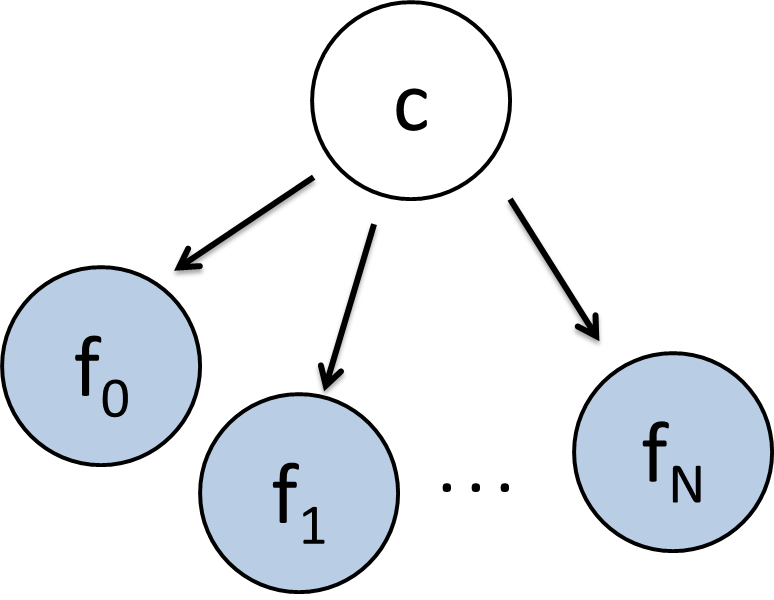
\includegraphics[width=.3\textwidth]{kmeansNB.png}
\centering
\caption{K-Means algorithm is the EM algorithm applied to this Bayes Net.}
\label{figure2}
\end{figure}


If we know that this is the strcuture of our bayes net, but we don't know any of the conditional probability distributions then we have to run Parameter Learning before we can run Inference.\\


In the dataset we are given, all the feature variables are observed (for each data point) but the class variable is hidden. Since we are running Parameter Learning on a bayes net where some variables are unobserved, we should use EM.\\


Lets review EM. In EM, you randomly initialize your model parameters, then you alternate between (E) assigning values to hidden variables, based on parameters and (M) computing parameters based on fully observed data.\\


\textbf{E-Step}: Coming up with values to hidden variables, based on parameters. If you work out the math of chosing the best values for the class variable based on the features of a given piece of data in your data set, it comes out to "for each data-point, chose the centroid that it is closest to, by euclidean distance, and assign that centroid's label." The proof of this is within your grasp! See lecture.\\


\textbf{M-Step}: Coming up with parameters, based on full assignments. If you work out the math of chosing the best parameter values based on the features of a given piece of data in your data set, it comes out to "take the mean of all the data-points that were labeled as c."\\


So what? Well this gives you an idea of the qualities of k-means. Like EM, it is provably going to find a local optimum. Like EM, it is not necessarily going to find a global optimum. It turns out those random initial values do matter.\\

\subsection{Intuition}

Figure 1 shows k-means with a 2-dimensional feature vector (each point has two dimensions, an x and a y). In your applications, will probably be working with data that has a lot of features. In fact each data-point may be hundreds of dimensions. We can visualize clusters in up to 3 dimensions (see figure 3) but beyond that you have to rely on a more mathematical understanding.\\

\begin{figure}[H]
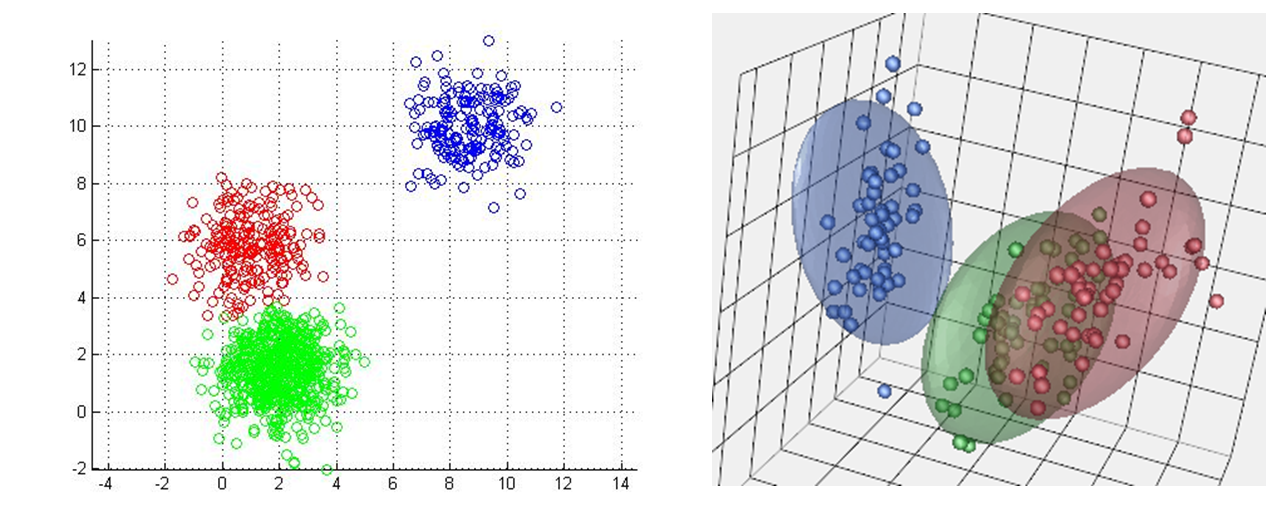
\includegraphics[width=.6\textwidth]{kmeans3d.png}
\centering
\caption{KMeans in other dimensions. (left) K-means in 2d. (right) K-means in 3d. You have to imagine k-means in 4d.}
\label{figure3}
\end{figure}


\section{Decision Tree}































\end{document}